\documentclass{sigchi}

% Use this section to set the ACM copyright statement (e.g. for
% preprints).  Consult the conference website for the camera-ready
% copyright statement.

% Copyright
\CopyrightYear{2020}
%\setcopyright{acmcopyright}
\setcopyright{acmlicensed}
%\setcopyright{rightsretained}
%\setcopyright{usgov}
%\setcopyright{usgovmixed}
%\setcopyright{cagov}
%\setcopyright{cagovmixed}
% DOI
\doi{http://dx.doi.org/10.475/123_4}
% ISBN
\isbn{123-4567-24-567/08/06}
%Conference
\conferenceinfo{CHI'16,}{May 07--12, 2016, San Jose, CA, USA}
%Price
\acmPrice{\$15.00}

% Use this command to override the default ACM copyright statement
% (e.g. for preprints).  Consult the conference website for the
% camera-ready copyright statement.

%% HOW TO OVERRIDE THE DEFAULT COPYRIGHT STRIP --
%% Please note you need to make sure the copy for your specific
%% license is used here!
% \toappear{
% Permission to make digital or hard copies of all or part of this work
% for personal or classroom use is granted without fee provided that
% copies are not made or distributed for profit or commercial advantage
% and that copies bear this notice and the full citation on the first
% page. Copyrights for components of this work owned by others than ACM
% must be honored. Abstracting with credit is permitted. To copy
% otherwise, or republish, to post on servers or to redistribute to
% lists, requires prior specific permission and/or a fee. Request
% permissions from \href{mailto:Permissions@acm.org}{Permissions@acm.org}. \\
% \emph{CHI '16},  May 07--12, 2016, San Jose, CA, USA \\
% ACM xxx-x-xxxx-xxxx-x/xx/xx\ldots \$15.00 \\
% DOI: \url{http://dx.doi.org/xx.xxxx/xxxxxxx.xxxxxxx}
% }

% Arabic page numbers for submission.  Remove this line to eliminate
% page numbers for the camera ready copy
% \pagenumbering{arabic}

% Load basic packages
\usepackage{balance}       % to better equalize the last page
\usepackage{graphics}      % for EPS, load graphicx instead 
\usepackage[T1]{fontenc}   % for umlauts and other diaeresis
\usepackage{txfonts}
\usepackage{mathptmx}
\usepackage[pdflang={en-US},pdftex]{hyperref}
\usepackage{color}
\usepackage{booktabs}
\usepackage{textcomp}

% Some optional stuff you might like/need.
\usepackage{microtype}        % Improved Tracking and Kerning
% \usepackage[all]{hypcap}    % Fixes bug in hyperref caption linking
\usepackage{ccicons}          % Cite your images correctly!
% \usepackage[utf8]{inputenc} % for a UTF8 editor only

% If you want to use todo notes, marginpars etc. during creation of
% your draft document, you have to enable the "chi_draft" option for
% the document class. To do this, change the very first line to:
% "\documentclass[chi_draft]{sigchi}". You can then place todo notes
% by using the "\todo{...}"  command. Make sure to disable the draft
% option again before submitting your final document.
\usepackage{todonotes}

% Paper metadata (use plain text, for PDF inclusion and later
% re-using, if desired).  Use \emtpyauthor when submitting for review
% so you remain anonymous.
\def\plaintitle{Show the proposed algorithm has the claimed running time by making all the computer verification explicit}
\def\plainauthor{First Author, Second Author, Third Author,
  Fourth Author, Fifth Author, Sixth Author}
\def\emptyauthor{}
\def\plainkeywords{\#SAT; \#2SAT; graph theory; complexity theory}
\def\plaingeneralterms{Documentation, Standardization}

% llt: Define a global style for URLs, rather that the default one
\makeatletter
\def\url@leostyle{%
  \@ifundefined{selectfont}{
    \def\UrlFont{\sf}
  }{
    \def\UrlFont{\small\bf\ttfamily}
  }}
\makeatother
\urlstyle{leo}

% To make various LaTeX processors do the right thing with page size.
\def\pprw{8.5in}
\def\pprh{11in}
\special{papersize=\pprw,\pprh}
\setlength{\paperwidth}{\pprw}
\setlength{\paperheight}{\pprh}
\setlength{\pdfpagewidth}{\pprw}
\setlength{\pdfpageheight}{\pprh}

% Make sure hyperref comes last of your loaded packages, to give it a
% fighting chance of not being over-written, since its job is to
% redefine many LaTeX commands.
\definecolor{linkColor}{RGB}{6,125,233}
\hypersetup{%
  pdftitle={\plaintitle},
% Use \plainauthor for final version.
%  pdfauthor={\plainauthor},
  pdfauthor={\emptyauthor},
  pdfkeywords={\plainkeywords},
  pdfdisplaydoctitle=true, % For Accessibility
  bookmarksnumbered,
  pdfstartview={FitH},
  colorlinks,
  citecolor=black,
  filecolor=black,
  linkcolor=black,
  urlcolor=linkColor,
  breaklinks=true,
  hypertexnames=false
}

% create a shortcut to typeset table headings
% \newcommand\tabhead[1]{\small\textbf{#1}}

% End of preamble. Here it comes the document.
\begin{document}

\title{\plaintitle}

\numberofauthors{3}
\author{%
  \alignauthor{Yinan Yang\\
    \affaddr{Unicersity of Bristol}\\
    \affaddr{Bristol, UK}\\
    \email{ff19085@bristol.ac.uk}}\\
  \alignauthor{John Lapinskas\\
   \affaddr{Unicersity of Bristol}\\
   \affaddr{Bristol, UK}\\
    \email{john.lapinskas@bristol.ac.uk}}\\
 
}

\maketitle

\begin{abstract}
  This project will carry out the process of theoretical reproduction in the field of algorithms. This project will focus on the field of \#2SAT. It will design a complete computerized validation process for that paper against the theories from previous important papers by prominent contributors in the field. Since there are few papers in the field that explains the reasoning process in detail, a large number of calculations and inferences are embedded in theorems. Therefore, sharing codes that reproduce the reasoning process is more challenging. This is not only a validation of the work of previous eminent workers in the field but also lays the foundation for later readers and learners in the field to avoid the appearance of repetition due to a large and cumbersome computational process. This is why it is essential to produce a complete computer verification.
  
  This project will simulate the workflow of an oracle machine through computer code, replicate the recursive logic of the paper, and accurately reduce a large number of branches in the paper to a solvable level through recursive algorithms. Verify the correctness of the thesis results by classifying the branch results in each case to determine if they are consistent with the original thesis results.
  
  On hardware systems, with the development of computer computing power, the amount of computing that was previously not readily available has become very easy. Thus the recursive calculations also become more reproducible than when the original paper was published. This also provides the hardware basis for the conduct of this project.
  
  For the evaluation of the validation of the results, since this project is a factual validation of existing theories, the results are compared according to the original thesis. If the results are entirely consistent, it is proved that the results are accurate in the original hypothesis, thus also proving the correctness of the original theory. If the results are not entirely consistent, then both the accuracy of the results of this project and the accuracy of the original theory need to be checked.
  
\end{abstract}

\category{H.5.m.}{Information Interfaces and Presentation
  (e.g. HCI)}{Miscellaneous} \category{See
  \url{http://acm.org/about/class/1998/} for the full list of ACM
  classifiers. This section is required.}{}{}

\keywords{\plainkeywords}

\section{Introduction}
First, the project will design a computer validation process of Magnus Wahlström's work in 2004.\cite{10.1016/j.tcs.2004.10.037} This project will focus on the \#2-SAT area of the algorithm domain, which will be covered in detail later in this introduction.

Most algorithm designs are algorithm designs for decision problems. For example, to find a solution that makes a Boolean formula satisfying. By finding a satisfying answer to a Boolean expression, we mean that given an arbitrary Boolean expression, such as $A \vee B $, one of the solutions that can make its result to be true if A is true, and B is true. This is the SAT question in the algorithmic field. SAT is the first issue that was demonstrated to be NP-complete.\cite{10.1145/800157.805047} As we all know, P-class is a fundamental complexity class that is verifiable by a deterministic Turing machine. However, NP is a generalization of P, which the lesson of choice problems decidable by a non-deterministic Turing machine that runs in polynomial time. A decisive question that is NP-complete means that it is complete for NP, which means that any question that is NP can be reduced to it in polynomial time.

Let us go back to the SAT problem. Going further, we will not only be content to find out if we can satisfy a particular Boolean expression, but we are trying to find out exactly how many solutions can satisfy that expression. This is the \#SAT question, brought up by Valiant in 1979.\cite{10.1016/0304-3975(79)90044-6} Valiant, meanwhile, raised the issue that this is a \#P-complete.

To find the final solution to a complete Boolean expression, we split out each of the propositional variables. Each propositional variable can contain either true or false. We define a literal to denote both a propositional variable x and its negation ¬x. A disjunction of literals is defined as a clause. And a conjunctive nurmal form, short for CNF, is a conjunction of clauses.

So we can represent some special case SAT questions, such as if each clause contains at most 2 literals, then we call this formula a 2-SAT formula. A more general representation is that if each clause contains at most no more than k literals in a hypothetical CNF, then we call it a k\-SAT formula (k>0). The \#2-SAT question of concern for this project can then be expressed as: how many possible solutions are there to make the formula satisfy a maximum of 2 liters per clause in any given proposed formula. Take for example the following.

\begin{align*}  
\left ( x_{0}\vee x_{1} \right )\wedge \left ( x_{1}\vee x_{2} \right )\wedge \left ( x_{2}\vee  x_{3} \right )\wedge \left ( x_{4}\right )
\end{align*}


Since we cannot give specific conclusions for all Boolean expressions, and indeed it is impossible, in this research area, we usually design a computational model to calculate the time complexity O of this model method. The time complexity usually describes the running time of an algorithm in a worst-case scenario. Computational models get different results in many branches, and we usually verify the worst time complexity to determine the time complexity of this algorithm.

In this project, the \#2SAT algorithm is explored from the initial upper bound of $ O\left ( 2^{n} \right )$, as proposed by Dubois, Zhang, Littman, and Dahllöf\cite{10.1007/3-540-45655-4_57} et al. The scheme is continuously optimized to propose $ O\left ( 1.3247^{n} \right )$, until this paper we forced uses the computer-verified work of Magnus Wahlström, who accelerated the algorithmic model of \#2SAT to $ O\left ( 1.2561^{n} \right )$ in 2004\cite{10.1016/j.tcs.2004.10.037}.

However, research in this field is purely theoretical, and the literature and papers are full of mathematical expressions and model reasoning. Papers in this field do not usually provide a specific computer code reproduction process for the given model, a process that is often hidden in the deductions of formulas, and it is difficult for later readers to rely solely on this paper to reproduce the full process of deductions. Moreover, as the theoretical research progresses, the inability to replicate the work of previously distinguished practitioners will have a very significant impact on subsequent research.

A survey of previous research in the field found that theory proponents tend to present only descriptions of algorithmic models, which in turn mostly use recursive algorithms, a method of solving problems by repeatedly decomposing them into subproblems of the same kind. The advantage of recursive algorithms is that they often effectively divide significant branching problems into small branching problems, and then solve them by targeting each branching problem that can be effectively focused on. However, recursive algorithms also have an irreparable disadvantage, if the recursive algorithm is simulated manually and the results are calculated manually, this leads to a considerable amount of computation, making it difficult or even impossible for later readers to verify the correctness of the reasoning process.

With the refinement of computer science and programming languages, we now can use more sophisticated language tools to refine the verification recursion problem. Moreover, with the increase in computer computing power in recent years, running large-scale recursion is no longer difficult. So both the theoretical basis and the hardware facilities were prepared for this project.

So an experimental replication of the reasoning process in this area of research will be very necessary. This is not only an experimental corroboration of the important theories of previous distinguished contributors but also an important reference for future continuing researchers in the field.

The project will be conducted based on the reading and validation of the thesis, which involves the validation of the different branches of Wahlström's work. (See Gantt chart). The initial design will be organized into a brief thesis validation report in the form of an algorithmic code design ensemble and proof draft, followed by specific code writing and validation.

As for the software required, python and related computing packages will be selected for this project because of the simplicity and ease of writing python. Due to the special nature of this project, the project does not require the operational efficiency of a complete project, only the verification of results, and therefore python has the advantage over c and java. The latest version of 3.8.2 will be chosen because the project will provide as much as possible a reasonable interpretation of previous outstanding work for future researchers in the field, so choosing the latest version of python will avoid creating a gap for future readers. As for the hardware part, since this project is a reproduction of a theoretical research example, there are no special hardware equipment requirements, just a computer that can run python.

A trial prototype will be made in June (see Gantt chart). In order to test our hypothesis, we will conduct quantitative and qualitative evaluations. Since the proof inference contains numerous branches, a defined structure will be designed for each branch to obtain the final result. We also hope to obtain predicted results from the computational model by randomly generating Boolean expressions to assess the validity of the computationally validated model that we produced.

The evaluation criteria will be determined by the degree of branching that completes the validation. Since the papers that we need to compute validation have numerous branches, we need to validate them item by item. If the results of the paper we verify are all correct, then the results of the calculations in all branches should be the same as predicted by the process of theoretical reasoning. If the results are different through computer code validation, then we need to discuss whether there was a problem with our step-by-step approach or with the original theoretical work.

The evaluation criteria will be determined by the degree of branching that completes the validation. Since the paper we need to verify numerous branches computationally, we need to verify the reasonableness of each branch item by item, comparing the results of the computational branches with the results of the original paper. If the results of the paper we verify are all correct, then the results of the calculations in all branches should be the same as predicted by the process of theoretical reasoning. If the results are different through computer code validation, then we need to discuss whether there was a problem with our step-by-step approach or with the original theoretical work.

\section{Literature Review}
Algorithms on counting problems had continued to evolve since the 1860s when Ryser proposed the first counting algorithm\cite{10.1017/s0013091500011299}, and Ryser pioneered the counting problem algorithm by proposing a time complexity of A for counting perfectly matched numbers in a binary graph. In the late 1870s, Valiant concluded that the complexity of the counting problem makes it a \#P class problem and can be statute as a \#P problem, so it is a \#P-complete problem\cite{10.1016/0304-3975(79)90044-6}.

Further, in the work of Magnus Wahlstrom et al. in 2004, they designed a computational model that reduced the temporal complexity of \#2SAT to  $ O\left ( 1.2561^{n} \right )$ \cite{10.1016/j.tcs.2004.10.037}., which is a great achievement. In this mathematical model, they designed a set of weights to measure the impact of each branch in the CNF on the final result. Under the influence of such a weighting model, the CNF can be continuously reduced by the recursive algorithm, thus speeding up the algorithm.This weighting model allows us to split a constraint graph into its dual connected components. Among other things, this provides a way to remove variables that appear only once in the formula during the polynomial time.On the other hand, the model can condense formula complexity into a single value containing the number of variables and variable clauses, which is more reflective of the complexity of a CNF than the original way of expressing formula complexity in numbers only, without regard to clause weights.

Since the main process of this project was to replicate the process of this paper and to simulate the validation with a computer program, our first task was to investigate what the technical line of this paper was. First let's introduce the computational tools and computational models he uses.

First of all, as introduced in the introduction above, the fundamental conceptual element of the field in which the project is located is literal, which contains either a variable $x$ or its negation $\neg x$. A clause is the disjunction of literals, and then the conjunction of multiple clauses forms the conjunction normal form, abbreviated to CNF. If each clause in a CNF contains up to k characters, we can call this CNF the k-SAT formula. For example.
\begin{center}
2-SAT:  $\left ( A \vee B \right )\wedge \left ( B \vee C \right ) $\\3-SAT:$\left ( A \vee B\vee C \right )\wedge \left ( B \vee C\vee D \right )$
\end{center}

In this paper, we define the degree $d\left( x \right)$ of a variable x in formula F as the number of clauses in $F$ containing $x$.
e.g.:in $\left ( A \vee B \right )\wedge \left ( B \vee C \right ) $ d$\left( B \right)$=2.
And the maximum degree of  any variable in F is d$\left(F\right)$, the number is $n_{d}\left ( F \right )$.\\
In this way, we get a method to measure formula complexity:\\
\begin{center}
	$m\left(F\right)=\sum_{x\in Var\left(F\right)} d\left(x\right)$
\end{center}
We define a model $M$ for $F$, a set L of all liters in $F$,and a weight vector $w$:\\
\begin{center}
$W\left ( M \right )=\sum_{\left \{ l\in L | l\;is\;true\;in\;M\right \}} w\left ( l \right )$\\
\end{center}
Be the same, we get a cardinality vector $c$ for $F$:\\
\begin{center}
$C\left ( M \right )=\prod_{\left \{ l\in L | l\;is\;true\;in\;M\right \}} c\left ( l \right )$\\
\end{center}
In this way, we get a weighted model  of F for \#2-SAT$\left(\#3-SAT\right)$:\\
\begin{center}
$\#2SAT_{w}(F, c, w)=\left ( \sum_{M\in S}C(M),W({M}') \right )$
\end{center}

At the same time, Magnus Wahlström introduced the concept of some graphs to illustrate the relationship between branches and branches better.Graphs are another way we look at Boolean expressions. We define a constraint graph of a formula:
\begin{center}
$\left \{ \left ( a,b \right ) |a\;and \;b\; occur \;together\;in\;at\;least\; one\;clause\right \}$
\end{center}
Connect: A formula F is connected iff in the corresponding constraint graph, there is a path from each variable to every other.As follow is a tree for 
\begin{center}
$\left ( A \vee B \right )\wedge \left ( B \vee C \right ) $:\\
\tikz \node {B}
child {node {A}}
child {node {C}};
\end{center}

Next, after the model style is built, we start calculating the temporal complexity of the branch.

\begin{center}
\tikz \node {v}
child {node {t1}}
child {node {t2}}
child {node {t3}}
child {node {t4}}
child {node {td}};
\end{center}
Think of a tree of formula. There is a node $v$ which has $d$ branches children. Each branch is labeled by recution complexity positive real number$\left(t_1,t_2...t_d\right)$ ,the branching number is the positive real-valued solution of
\begin{center}
	$\sum_{i=1}^{d} x^{-t_{i}}=1$
\end{center}
We defined the branching number of tuple
 $\left(t_1,t_2...t_d\right)$ is $\tau\left(t_1,t_2...t_d\right)$ ie. $\tau(4,4)\rightarrow x=\sqrt[4]{2}\approx 1.1892$

	In order to avoid the result deviation caused by the simplified formula, the prof formula is introduced, and the objective formula is simplified on the basis of increasing the weight.\\
\begin{enumerate}
\item If $F$ contains an empty clause then $F:=(\varnothing), c:=0$ and $w:=0$
\item If there is a clause $(1 \vee \ldots),$ then it is removed. If any variable $a$ thereby gets removed then there are three cases:
(a) If $w(a)=w(\neg a)$ then $c:=c \cdot(c(a)+c(\neg a)) ; w:=w+w(a)$\\
(b) If $w(a)<w(\neg a)$ then $c:=c \cdot c(\neg a) ; w:=w+w(\neg a)$\\
(c) If $w(a)>w(\neg a)$ then $c:=c \cdot c(a) ; w:=w+w(a)$
\item If there is a clause $(0 \vee \ldots),$ then 0 is removed from it.
\item If there is a clause $(a),$ then it is removed and $c:=c \cdot c(a), w:=w+w(a) .$ If $a$ still appears in $F$ then $F:=F[a=1]$
\item If there are two clauses $x=\left(a \vee b \vee a^{\prime}\right), y=(a \vee b)$ then remove $x$. If the variable $a^{\prime}$ thereby gets removed then handle it as in case 2 .
\end{enumerate}
After some steps of simplification and proof we get Lemma 1:\\
\begin{quote}[Lemma 1]
$Let({F}',c,w)=Prop(F,c,w)\\and\;({c}',{w}')=\#2SAT_{w}({F}',c,w).\\
Then\; \#2SATw(F ,c,w)=(c*{c}',w+{w}')$.
\end{quote}

In order to simplify the formula $F$, we have $F_{1}$, $F_{2}$, such that \\$Var(F_{1})\bigcap Var(F_2)=\left \{ v \right \} $.
\begin{enumerate} 
\item Let $\left(c_{t}, w_{t}\right)=\# 2 S A T_{w}\left(F_{1}[v=1], \mathbf{c}, \mathbf{w}\right)$ and $\left(c_{f}, w_{f}\right)=\# 2 S A T_{w}\left(F_{1}[v=0], \mathbf{c}, \mathbf{w}\right)$
\item Modify c and $\mathbf{w}$ so that $c(v) \leftarrow c_{t} \cdot c(v), c(\neg v) \leftarrow c_{f} \cdot c(\neg v), w(v) \leftarrow w_{t}+w(v)$ and
$w(\neg v) \leftarrow w_{f}+w(\neg v)$
\item Finally, return $\# 2 \operatorname{SAT}_{w}\left(F_{2}, \mathbf{c}, \mathbf{w}\right)$
\end{enumerate}
This procedure is to remove $F_1$ by multiplier reduction. And we get Lemma 2:
\begin{quote}[Lemma 2]
Applying multiplier reduction does not change the return value of $\#2SAT w (F, c, w)$.
\end{quote}

	According to Lemma 1 and Lemma 2, we can naturally get Lemma 3:
\begin{quote}[Lemma 3]
	The result of recursively branching on the variable $v$ in the formula $F$ equals $\#2SAT_{w}(F, c, w)$.
\end{quote}

Since $d(F)$ is discrete, it is discussed in three cases:
\begin{enumerate}
	\item the main function: $d(F)>5$
	\item help function1 $4<=d(F)<=5$
	\item help function2 $d(F)<=3$
\end{enumerate}
	At First, we need to solve the $C_{3}(F,c,w)$.Algorithm $C_{3}(F, \mathbf{c}, \mathbf{w})$ as follow:
\begin{enumerate}	
	\item Case 1: If $F$ contains no clauses, return (1, 0). If $F$ contains an empty clause, return (0, 0).\
	\item Case 2: If $F$ is not connected, return $(c, w)$ where $c=\prod_{i=0}^{j} c_{i}, w=\sum_{i=0}^{j} w_{i}$ and $\left(c_{i}, w_{i}\right)=C\left(F_{i}, \mathbf{c}, \mathbf{w}\right)$ for the connected components $F_{0}, \ldots, F_{j}$
	\item Case 3: If multiplier reduction applies, apply it, removing the part with lowest $n_{3}(F)$ value.
	\item Case 4: If $d(F)=3,$ pick a variable $x, d(x)=3,$ with as many neighbours of degree 3 as possible, and recursively branch on it. Otherwise, recursively branch on any variable.$  $
\end{enumerate}
By calling the loop recursively, we could get Lemma 5.
\begin{quote}[Lemma 5]
	$C_{3}(F ,c,w)$runs in $O(ploy(n)*\tau(4,4)^{n_{3}(F))})$\\time, where $p(n)$ is a polynomial in $n$.
\end{quote}

In the same way, we can get	algorithm $C_{5}(F, \mathbf{c}, \mathbf{w})$
\begin{enumerate}
	\item Case 1: If $F$ contains no clauses, return (1, 0). If $F$ contains an empty clause, return (0, 0).
	\item Case 2: If $F$ is not connected, return $(c, w)$ where $c=\prod_{i=0}^{j} c_{i}, w=\sum_{i=0}^{j} w_{i}$ and $\left(c_{i}, w_{i}\right)=C\left(F_{i}, \mathbf{c}, \mathbf{w}\right)$ for the connected components $F_{0}, \ldots, F_{j}$
	\item Case 3: If $d(F)<4,$ return $C_{3}(F, \mathbf{c}, \mathbf{w})$ 
	\item Case 4: If multiplier reduction applies, apply it, removing the part with lowest $f(F)$ value.
	\item Case 5: Pick a variable $x$ of maximum degree such that $S(x)$ is maximized. (a) If $N(x)$ is connected to the rest of the graph through only 2 external vertices $y, z$ such that $d(y) \geqslant d(z)$ then branch on $y .$
	(b) Otherwise, branch on $x .$
	$S(x)=\sum_{y \in N(x)} d(y)$
\end{enumerate}
From the quotient of the complexity of the formula and the maximum number of branches, it can be inferred that the larger the quotient, the greater the time complexity of the worst case.\\So discuss the worst case of C5 in the value range of linear function $f\left(n,m\right)$, where $n=n(F)$ and $m=m(F)$. \\
We need a sequence of worst cases as the $m / n$ quotient increases, and with each worst case we associate a linear function $f_{i}(n, m)=a_{i} n+b_{i} m$. \\
$\begin{aligned} f(n, m) &=f_{i}(n, m) \text { if } k_{i}<m / n \leqslant k_{i+1}, \quad 0 \leqslant i \leqslant 9 \\ f_{i}(n, m) &=\chi_{i} n+\left(m-k_{i} n\right) b_{i}, \quad 0 \leqslant i \leqslant 9 \\ \chi_{0} &=0 \\ \chi_{i} &=\chi_{i-1}+\left(k_{i}-k_{i-1}\right) b_{i-1}, \quad 1 \leqslant i \leqslant 10 \\ a_{i} &=\chi_{i}-k_{i} b_{i} \end{aligned}$\\

\begin{center}
	$T_{a b}$
	$k_{i}, \chi_{i}$ and running times \\
	\begin{tabular}{llll}
		\hline$i$ & $k_{i}$ & $\chi_{i}$ & Running time \\
		\hline 0 & 0 & 0 & $\mathrm{O}(1)$ \\
		1 & 2 & 0 & $\mathrm{O}(p o l y(n))$ \\
		2 & 3 & 1& $\mathrm{O}\left(1.1892^{n}\right)$ \\
		3 & 3.5 &1.1340& $\mathrm{O}\left(1.2172^{n}\right)$ \\
		4 & 3.75&1.1914 & $0\left(1.2294^{n}\right)$ \\
		5 & 4 & 1.2410&$0\left(1.2400^{n}\right)$ \\
		6 & $4+4 / 29$ & 1.2536& $0\left(1.2427^{n}\right)$ \\
		7 & $4+4 / 9$ &1.2788& $0\left(1.2481^{n}\right)$ \\
		8 & $4+4 / 7$ &1.2881& $0\left(1.2481^{n}\right)$ \\
		9 & 4.8 &1.3033& $0\left(1.2501^{n}\right)$ \\
		10 & 5 & 1.3154& $0\left(1.2534^{n}\right)$ \\
		\hline
	\end{tabular}\\
	
\end{center}

\begin{table*}
\begin{center}
	$b_{i}$ and $a_{i}$ parameters\\
\end{center}
	%\resizebox{\textwidth}{30mm}{
	\centering
		{
		\begin{tabular}{llll}
			\hline$i$ & $b_{i}$, definitions & $b_{i}$ & $a_{i}$ \\
			\hline 0 & 0 & 0 & 0 \\
			1 & 1 & 1 & $-2$ \\
			2 & $\tau\left(1+5 b_{2}, 5+5 b_{2}\right)=\tau(4,4)$ & 0.2680 & 0.1961 \\
			3 & $\tau\left(\chi_{3}+4.5 b_{3}, 5 \chi_{3}+4.5 b_{3}\right)=\tau(4,4)$ & 0.2295 & 0.3308 \\
			4 & $\tau\left(\chi_{4}+4.25 b_{4}, 5 \chi_{4}+5.25 b_{4}\right)=\tau(4,4)$ & 0.1987 & 0.4461 \\
			5 & $\tau\left(\chi_{5}+6 b_{5}, 6 \chi_{5}+2 b_{5}\right)=\tau(4,4)$ & 0.0914 & 0.8755 \\
			6 & $\tau\left(\chi_{6}+(5+25 / 29) b_{6}, 6 \chi_{6}+(3+5 / 29) b_{6}\right)=\tau(4,4)$ & 0.0821 & 0.9139 \\
			7 & $\tau\left(\chi_{7}+(5+5 / 9) b_{7}, 6 \chi_{7}+(3+1 / 3) b_{7}\right)=\tau(4,4)$ & 0.0736 & 0.9517 \\
			8 & $\tau\left(\chi_{8}+(5+3 / 7) b_{8}, 6 \chi_{8}+(4+4 / 7) b_{8}\right)=\tau(4,4)$ & 0.0665 & 0.9841 \\
			9 & $\tau\left(\chi_{9}+5.2 b_{9}, 6 \chi_{9}+5.2 b_{9}\right)=\tau(4,4)$ & 0.0602 & 1.0143 \\
			\hline
	\end{tabular}}
\end{table*}

 We have got $a_{i},b_{i},k_{i}$. We need a lemma that allows us to make a connection between the value of m(F )/n(F ) and worst-case branchings.
\begin{quote}[Lemma 6]
	Let $F$ be a non-empty formula such that $m(F) / n(F)=k,$ and define $\alpha(x)$ and
	$\beta(x)$ such that
	$$
	\begin{aligned}
	\alpha(x) &=d(x)+|\{y \in N(x) | d(y)<k\}| \\
	\beta(x) &=1+\sum_{\{y \in N(x) | d(y)<k\}} 1 / d(y)
	\end{aligned}
	$$
	There exists some variable $x \in \operatorname{Var}(F)$ with $d(x) \geqslant k$ such that $\alpha(x) / \beta(x) \geqslant k$
\end{quote}
We will need to prove that the worst-case branching number in each section is $\tau(4,4)$. For different ranges of m/n values, we need to show that when $m/n\leqslant5$, the time complexity is less than $\mathrm{O}\left(1.2561^{n}\right)$. So we broke down a number of situations.
\begin{enumerate}
	\item Case: $m / n \leqslant2$
		\item Case: $m / n \in[2,3]$
	\item Case: $d(F)=5$ which gets a branching number less than $\tau(4,4)$.
	\item Case: $m / n \in[3,3.5], d(F)=4$
	\item Case: $m / n \in[3.5,3.75], d(F)=4$
	\item Case: $ m / n \in[3.75,4], d(F)=4 .$ 
	\item Case:  $m / n \in[4,4+4 / 29]$
	\item Case: $m / n \in[4+4 / 29,4+4 / 9]$
	\item Case: $m / n \in[4+4 / 9,4+4 / 7]$
	\item Case: $m / n \in[4+4 / 7,4.8]$
	\item Case: $m / n \in[4.8,5]$
\end{enumerate}
After all of the above branches have been recursively calculated, we can deduce the conclusion.
\begin{quote}[Theorem 11]
	$C(F, \mathbf{c}, \mathbf{w})$ runs in $\mathrm{O}\left(1.2561^{n}\right)$ time.
\end{quote}
\section{Typeset Text}
The styles contained in this document have been modified from the
default styles to reflect ACM formatting conventions. For example,
content paragraphs like this one are formatted using the Normal style.

\LaTeX\ sometimes will create overfull lines that extend into columns.
To attempt to combat this, the \texttt{.cls} file has a command,
\texttt{{\textbackslash}sloppy}, that essentially asks \LaTeX\ to
prefer underfull lines with extra whitespace.  For more details on
this, and info on how to control it more finely, check out
{\url{http://www.economics.utoronto.ca/osborne/latex/PMAKEUP.HTM}}.

\subsection{Title and Authors}

Your paper's title, authors and affiliations should run across the
full width of the page in a single column 17.8 cm (7 in.) wide.  The
title should be in Helvetica or Arial 18-point bold.  Authors' names
should be in Times New Roman or Times Roman 12-point bold, and
affiliations in 12-point regular.  

See \texttt{{\textbackslash}author} section of this template for
instructions on how to format the authors. For more than three
authors, you may have to place some address information in a footnote,
or in a named section at the end of your paper. Names may optionally
be placed in a single centered row instead of at the top of each
column. Leave one 10-point line of white space below the last line of
affiliations.

\subsection{Abstract and Keywords}

Every submission should begin with an abstract of about 150 words,
followed by a set of Author Keywords and ACM Classification
Keywords. The abstract and keywords should be placed in the left
column of the first page under the left half of the title. The
abstract should be a concise statement of the problem, approach, and
conclusions of the work described. It should clearly state the paper's
contribution to the field of HCI\@.

\subsection{Normal or Body Text}

Please use a 10-point Times New Roman or Times Roman font or, if this
is unavailable, another proportional font with serifs, as close as
possible in appearance to Times Roman 10-point. Other than Helvetica
or Arial headings, please use sans-serif or non-proportional fonts
only for special purposes, such as source code text.

\subsection{First Page Copyright Notice}
This template include a sample ACM copyright notice at the bottom of
page 1, column 1.  Upon acceptance, you will be provided with the
appropriate copyright statement and unique DOI string for publication.
Accepted papers will be distributed in the conference
publications. They will also be placed in the ACM Digital Library,
where they will remain accessible to thousands of researchers and
practitioners worldwide. See
\url{http://acm.org/publications/policies/copyright_policy} for the
ACM's copyright and permissions policy.

\subsection{Subsequent Pages}

On pages beyond the first, start at the top of the page and continue
in double-column format.  The two columns on the last page should be
of equal length.

\begin{figure}
\centering
  
\includegraphics[width=0.9\columnwidth]{figures/sigchi-logo}
  \caption{Insert a caption below each figure. Do not alter the
    Caption style.  One-line captions should be centered; multi-line
    should be justified. }~\label{fig:figure1}
\end{figure}

\subsection{References and Citations}

Use a numbered list of references at the end of the article, ordered
alphabetically by last name of first author, and referenced by numbers
in
brackets~\cite{acm_categories,ethics,Klemmer:2002:WSC:503376.503378}.
Your references should be published materials accessible to the
public. Internal technical reports may be cited only if they are
easily accessible (i.e., you provide the address for obtaining the
report within your citation) and may be obtained by any reader for a
nominal fee. Proprietary information may not be cited. Private
communications should be acknowledged in the main text, not referenced
(e.g., ``[Borriello, personal communication]'').

References should be in ACM citation format:
\url{http://acm.org/publications/submissions/latex_style}. This
includes citations to internet
resources~\cite{acm_categories,cavender:writing,CHINOSAUR:venue,psy:gangnam}
according to ACM format, although it is often appropriate to include
URLs directly in the text, as above.


% Use a numbered list of references at the end of the article, ordered
% alphabetically by first author, and referenced by numbers in
% brackets~\cite{ethics, Klemmer:2002:WSC:503376.503378,
%   Mather:2000:MUT, Zellweger:2001:FAO:504216.504224}. For papers from
% conference proceedings, include the title of the paper and an
% abbreviated name of the conference (e.g., for Interact 2003
% proceedings, use \textit{Proc. Interact 2003}). Do not include the
% location of the conference or the exact date; do include the page
% numbers if available. See the examples of citations at the end of this
% document. Within this template file, use the \texttt{References} style
% for the text of your citation.

% Your references should be published materials accessible to the
% public.  Internal technical reports may be cited only if they are
% easily accessible (i.e., you provide the address for obtaining the
% report within your citation) and may be obtained by any reader for a
% nominal fee.  Proprietary information may not be cited. Private
% communications should be acknowledged in the main text, not referenced
% (e.g., ``[Robertson, personal communication]'').

\begin{table}
  \centering
  \begin{tabular}{l r r r}
    % \toprule
    & & \multicolumn{2}{c}{\small{\textbf{Test Conditions}}} \\
    \cmidrule(r){3-4}
    {\small\textit{Name}}
    & {\small \textit{First}}
      & {\small \textit{Second}}
    & {\small \textit{Final}} \\
    \midrule
    Marsden & 223.0 & 44 & 432,321 \\
    Nass & 22.2 & 16 & 234,333 \\
    Borriello & 22.9 & 11 & 93,123 \\
    Karat & 34.9 & 2200 & 103,322 \\
    % \bottomrule
  \end{tabular}
  \caption{Table captions should be placed below the table. We
    recommend table lines be 1 point, 25\% black. Minimize use of
    table grid lines.}~\label{tab:table1}
\end{table}

\section{Sections}

The heading of a section should be in Helvetica or Arial 9-point bold,
all in capitals. Sections should \textit{not} be numbered.

\subsection{Subsections}

Headings of subsections should be in Helvetica or Arial 9-point bold
with initial letters capitalized.  For sub-sections and
sub-subsections, a word like \emph{the} or \emph{of} is not
capitalized unless it is the first word of the heading.

\subsubsection{Sub-subsections}

Headings for sub-subsections should be in Helvetica or Arial 9-point
italic with initial letters capitalized.  Standard
\texttt{{\textbackslash}section}, \texttt{{\textbackslash}subsection},
and \texttt{{\textbackslash}subsubsection} commands will work fine in
this template.

\section{Figures/Captions}

Place figures and tables at the top or bottom of the appropriate
column or columns, on the same page as the relevant text (see
Figure~\ref{fig:figure1}). A figure or table may extend across both
columns to a maximum width of 17.78 cm (7 in.).

\begin{figure*}
  \centering
  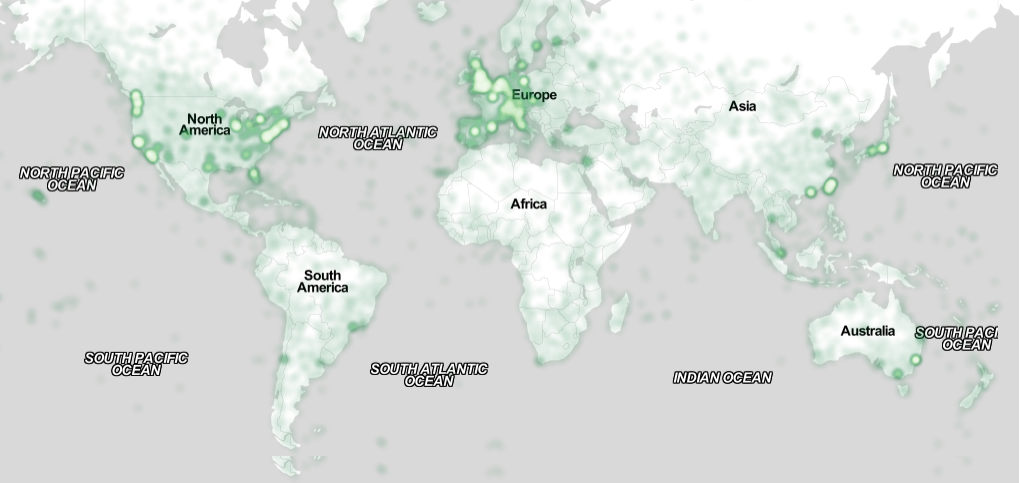
\includegraphics[width=1.75\columnwidth]{figures/map}
  \caption{In this image, the map maximizes use of space. You can make
    figures as wide as you need, up to a maximum of the full width of
    both columns. Note that \LaTeX\ tends to render large figures on a
    dedicated page. Image: \ccbynd~ayman on
    Flickr.}~\label{fig:figure2}
\end{figure*}

Captions should be Times New Roman or Times Roman 9-point bold.  They
should be numbered (e.g., ``Table~\ref{tab:table1}'' or
``Figure~\ref{fig:figure1}''), centered and placed beneath the figure
or table.  Please note that the words ``Figure'' and ``Table'' should
be spelled out (e.g., ``Figure'' rather than ``Fig.'') wherever they
occur. Figures, like Figure~\ref{fig:figure2}, may span columns and
all figures should also include alt text for improved accessibility.
Papers and notes may use color figures, which are included in the page
limit; the figures must be usable when printed in black-and-white in
the proceedings.

The paper may be accompanied by a short video figure up to five
minutes in length. However, the paper should stand on its own without
the video figure, as the video may not be available to everyone who
reads the paper.  

\subsection{Inserting Images}
When possible, include a vector formatted graphic (i.e. PDF or EPS).
When including bitmaps,  use an image editing tool to resize the image
at the appropriate printing resolution (usually 300 dpi).

\section{Quotations}
Quotations may be italicized when \textit{``placed inline''} (Anab,
23F).

\begin{quote}
Longer quotes, when placed in their own paragraph, need not be
italicized or in quotation marks when indented (Ramon, 39M).  
\end{quote}

\section{Language, Style, and Content}

The written and spoken language of SIGCHI is English. Spelling and
punctuation may use any dialect of English (e.g., British, Canadian,
US, etc.) provided this is done consis- tently. Hyphenation is
optional. To ensure suitability for an international audience, please
pay attention to the following:

\begin{itemize}
\item Write in a straightforward style.
\item Try to avoid long or complex sentence structures.
\item Briefly define or explain all technical terms that may be
  unfamiliar to readers.
\item Explain all acronyms the first time they are used in your
  text---e.g., ``Digital Signal Processing (DSP)''.
\item Explain local references (e.g., not everyone knows all city
  names in a particular country).
\item Explain ``insider'' comments. Ensure that your whole audience
  understands any reference whose meaning you do not describe (e.g.,
  do not assume that everyone has used a Macintosh or a particular
  application).
\item Explain colloquial language and puns. Understanding phrases like
  ``red herring'' may require a local knowledge of English.  Humor and
  irony are difficult to translate.
\item Use unambiguous forms for culturally localized concepts, such as
  times, dates, currencies, and numbers (e.g., ``1--5--97'' or
  ``5/1/97'' may mean 5 January or 1 May, and ``seven o'clock'' may
  mean 7:00 am or 19:00). For currencies, indicate equivalences:
  ``Participants were paid {\fontfamily{txr}\selectfont \textwon}
  25,000, or roughly US \$22.''
\item Be careful with the use of gender-specific pronouns (he, she)
  and other gendered words (chairman, manpower, man-months). Use
  inclusive language that is gender-neutral (e.g., she or he, they,
  s/he, chair, staff, staff-hours, person-years). See the
  \textit{Guidelines for Bias-Free Writing} for further advice and
  examples regarding gender and other personal
  attributes~\cite{Schwartz:1995:GBF}. Be particularly aware of
  considerations around writing about people with disabilities.
\item If possible, use the full (extended) alphabetic character set
  for names of persons, institutions, and places (e.g.,
  Gr{\o}nb{\ae}k, Lafreni\'ere, S\'anchez, Nguy{\~{\^{e}}}n,
  Universit{\"a}t, Wei{\ss}enbach, Z{\"u}llighoven, \r{A}rhus, etc.).
  These characters are already included in most versions and variants
  of Times, Helvetica, and Arial fonts.
\end{itemize}

\section{Accessibility}
The Executive Council of SIGCHI has committed to making SIGCHI
conferences more inclusive for researchers, practitioners, and
educators with disabilities. As a part of this goal, the all authors
are asked to work on improving the accessibility of their
submissions. Specifically, we encourage authors to carry out the
following five steps:
\begin{enumerate}
\item Add alternative text to all figures
\item Mark table headings
\item Add tags to the PDF
\item Verify the default language
\item Set the tab order to ``Use Document Structure''
\end{enumerate}
For more information and links to instructions and resources, please
see: \url{http://chi2016.acm.org/accessibility}.  The
\texttt{{\textbackslash}hyperref} package allows you to create well tagged PDF files,
please see the preamble of this template for an example.

\section{Page Numbering, Headers and Footers}
Your final submission should not contain footer or header information
at the top or bottom of each page. Specifically, your final submission
should not include page numbers. Initial submissions may include page
numbers, but these must be removed for camera-ready. Page numbers will
be added to the PDF when the proceedings are assembled.

\section{Producing and Testing PDF Files}

We recommend that you produce a PDF version of your submission well
before the final deadline.  Your PDF file must be ACM DL
Compliant. The requirements for an ACM Compliant PDF are available at:
{\url{http://www.sheridanprinting.com/typedept/ACM-distilling-settings.htm}}.

Test your PDF file by viewing or printing it with the same software we
will use when we receive it, Adobe Acrobat Reader Version 10. This is
widely available at no cost. Note that most
reviewers will use a North American/European version of Acrobat
reader, so please check your PDF accordingly.

When creating your PDF from Word, ensure that you generate a tagged
PDF from improved accessibility. This can be done by using the Adobe
PDF add-in, also called PDFMaker. Select Acrobat | Preferences from
the ribbon and ensure that ``Enable Accessibility and Reflow with
tagged Adobe PDF'' is selected. You can then generate a tagged PDF by
selecting ``Create PDF'' from the Acrobat ribbon.

\section{Conclusion}

It is important that you write for the SIGCHI audience. Please read
previous years' proceedings to understand the writing style and
conventions that successful authors have used. It is particularly
important that you state clearly what you have done, not merely what
you plan to do, and explain how your work is different from previously
published work, i.e., the unique contribution that your work makes to
the field. Please consider what the reader will learn from your
submission, and how they will find your work useful. If you write with
these questions in mind, your work is more likely to be successful,
both in being accepted into the conference, and in influencing the
work of our field.

\section{Acknowledgments}

Sample text: We thank all the volunteers, and all publications support
and staff, who wrote and provided helpful comments on previous
versions of this document. Authors 1, 2, and 3 gratefully acknowledge
the grant from NSF (\#1234--2012--ABC). \textit{This whole paragraph is
  just an example.}

% Balancing columns in a ref list is a bit of a pain because you
% either use a hack like flushend or balance, or manually insert
% a column break.  http://www.tex.ac.uk/cgi-bin/texfaq2html?label=balance
% multicols doesn't work because we're already in two-column mode,
% and flushend isn't awesome, so I choose balance.  See this
% for more info: http://cs.brown.edu/system/software/latex/doc/balance.pdf
%
% Note that in a perfect world balance wants to be in the first
% column of the last page.
%
% If balance doesn't work for you, you can remove that and
% hard-code a column break into the bbl file right before you
% submit:
%
% http://stackoverflow.com/questions/2149854/how-to-manually-equalize-columns-
% in-an-ieee-paper-if-using-bibtex
%
% Or, just remove \balance and give up on balancing the last page.
%
\balance{}

\section{References Format}
Your references should be published materials accessible to the
public. Internal technical reports may be cited only if they are
easily accessible and may be obtained by any reader for a nominal
fee. Proprietary information may not be cited. Private communications
should be acknowledged in the main text, not referenced (e.g.,
[Golovchinsky, personal communication]). References must be the same
font size as other body text. References should be in alphabetical
order by last name of first author. Use a numbered list of references
at the end of the article, ordered alphabetically by last name of
first author, and referenced by numbers in brackets. For papers from
conference proceedings, include the title of the paper and the name of
the conference. Do not include the location of the conference or the
exact date; do include the page numbers if available. 

References should be in ACM citation format:
\url{http://www.acm.org/publications/submissions/latex_style}.  This
includes citations to Internet
resources~\cite{CHINOSAUR:venue,cavender:writing,psy:gangnam}
according to ACM format, although it is often appropriate to include
URLs directly in the text, as above. Example reference formatting for
individual journal articles~\cite{ethics}, articles in conference
proceedings~\cite{Klemmer:2002:WSC:503376.503378},
books~\cite{Schwartz:1995:GBF}, theses~\cite{sutherland:sketchpad},
book chapters~\cite{winner:politics}, an entire journal
issue~\cite{kaye:puc},
websites~\cite{acm_categories,cavender:writing},
tweets~\cite{CHINOSAUR:venue}, patents~\cite{heilig:sensorama}, 
games~\cite{supermetroid:snes}, and
online videos~\cite{psy:gangnam} is given here.  See the examples of
citations at the end of this document and in the accompanying
\texttt{BibTeX} document. This formatting is a edited version of the
format automatically generated by the ACM Digital Library
(\url{http://dl.acm.org}) as ``ACM Ref.'' DOI and/or URL links are
optional but encouraged as are full first names. Note that the
Hyperlink style used throughout this document uses blue links;
however, URLs in the references section may optionally appear in
black.

% BALANCE COLUMNS
\balance{}

% REFERENCES FORMAT
% References must be the same font size as other body text.
\bibliographystyle{SIGCHI-Reference-Format}
\bibliography{reference}

\end{document}

%%% Local Variables:
%%% mode: latex
%%% TeX-master: t
%%% End:
